\documentclass[twocolumn]{article}
\usepackage{amsmath, amssymb, graphicx, enumerate, cuted}

\renewcommand{\familydefault}{\sfdefault}

\title{Field Sampling}
\author{Purva Parmar \\ 20181081}
\date{}

\begin{document}

\graphicspath{{../}}
\setlength{\parindent}{0pt}
\setlength{\parskip}{\baselineskip}

\maketitle

\section{Aim}

To understand ecological sampling and do it to study florets and inflorescence

\section{Lab Report}
\subsection{Write-Up}

\begin{enumerate}[a)]
\item \textbf{Brief Description of the exercise of ecological sampling} 

Ecological Sampling is about picking out a sample from a large population to study some phenomenon. 

There is no rigid experimentation with heavy manipulation. It is about observing the happenings and extracting meaningful info.

We study a sample to understand the behaviours of a larger population. 

Since studying a large population is often impractical, it is important to choose samples in a proper way. The samples must resemble the distributions in population to a good extent. Else, we may have very biased results.

In this experiment, we studied florets and inflorescences. To sample the data, we marked out grids of regular sizes and counted things systematically in each grid. 

This sample is assumed to represent the bigger population of flowers out there.

\item \textbf{Difference between Samples and Populations}

Simply speaking, a Population is just the entire data-set. All the values that can possibly exist, form the Population. In a real world, this could refer to all the human beings, for example.


A sample is a smaller subset of the population. For example, the set of all students in IISER is a sample, a subset of all students in India.


It is often impractical to study a whole population. So, we pick out small samples to study, and apply statistical methods to draw conclusions about the larger population. 

\item \textbf{The utility of statistics in going from the sample to the population}

We are going to draw conclusions about a large population based on the studies done on a much smaller sample.

It is important that the sample is chosen randomly, so that it resembles the distributions seen in nature. 

We can then apply a lot of statistical tools, like Mean, Standard Deviation, Standard Error, Normal Distributions, etc. to draw conclusions about the Population from the Sample.

\item \textbf{Expected Results}

I expect both the white and purple flowers to be from the same respective populations. I do not see a reason why some grids should show a difference. They were all planted the same.


The inflorescences per grid may possibly be a Poisson. Tests to be done.

\end{enumerate}

\subsection{Plots} 

\textbf{Plot the distribution of fractional occurrences of the number of florets per inflorescence for}
\begin{enumerate}[a)]
    \item Purple-top
    \item Purple-side 
    \item White-top 
    \item White-side
\end{enumerate}
\textbf{and comment on their similarity or otherwise.}

The graph has been attached in a separate sheet.

So, the initial points are all very high, and then we see a more or less constant value of fractions and then, the fractions drop suddenly.


So, the whole graph has three stages:
\begin{itemize}
    \item Initial Stage of high fractional occurrences
    \item Middle Stage of a more or less constant fractional occurrence, from around 2-12 or 13 florets per inflorescence
    \item Final Stage of low fractional occurrences
\end{itemize}

Since florets spend their initial time as buds, the number corresponding to 0 florets shows the number of buds. 

It takes some time for the buds to grow into florets. So, there is a definite temporal component in the graph. 

The initial high stage shows some of the younglings. 

However, then we have a very broad middle stage. 

One possible explanation is that after the buds start to bloom, they randomly have some number of florets, lying in that broad range.

There is a low fraction with very high number of florets. These may be due to some special factors which rarely occur. Possibilities may include optimum resources for a large inflorescence, some genetic trait or maybe age. 

We do not yet know if there arise more florets as the flower ages. Larger data sets and studies with planned experiments can help figure out the reasons for the graph dividing into three different parts.

To conclude, the initial high stage corresponds to the young buds, which are yet to bloom. The middle broad constant stage may correspond just different numbers of florets per inflorescence that a flower can have. 

The final stage may correspond to either some old age survivorship, some genetic trait, or maybe just very favourable environmental conditions for the flower.

\subsubsection{t-test}

\textbf{Test for equality of population means for the above 4 categories}


Here are the relevant values, calculated from PAST. 


The population means are very very close to each other. The t-values are extremely small. 

This implies that all the flowers are from the same population and there is no statistical difference between any pair.

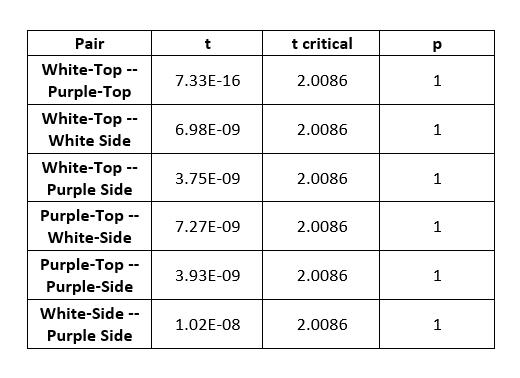
\includegraphics[width = \linewidth]{t-values.png}

\subsubsection{Poisson Distributions}

\textbf{Plot the distribution of fractional occurrences of the number of inflorescences per grid and check if they can be Poisson Distributions, for}
\begin{enumerate}[a)]
    \item Top grids
    \item Side grids 
\end{enumerate}

\begin{figure}[h]
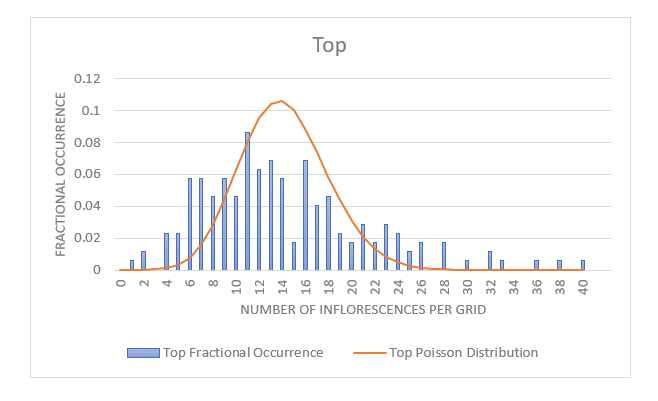
\includegraphics[width = \linewidth]{Top Poisson.png}
\caption{Top Grids}
\end{figure}

\begin{figure}[h]
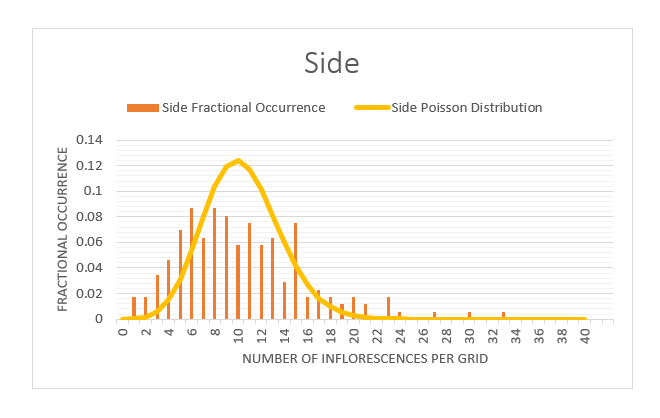
\includegraphics[width = \linewidth]{Side Poisson.png}
\caption{Side Grids}
\end{figure}


\begin{itemize}
    \item Mean of Top: 14.19 Inflorescences per Grid
    \item Mean of Side: 10.28 Inflorescences per Grid
\end{itemize}

The Top and Side Grids show, to some extent, a Poisson Distribution. But overall, it cuts off on the top. 

They appear to be Poisson with cuts and exceptions.

\end{document}